\chapter{The Bracelet}

The interactive bracelet consists mainly of an electronic ink display and several touch sensors for conscious interaction and a motion sensor for gesture recognition. The bracelet's design focuses on wearing comfort, low weight and small error of unintended activation.

\section{Manufacturing Techniques}

In this section, the various methods and tools used for designing and manufacturing the bracelet prototypes will be explained in detail.

\subsection{Computer Aided Design}
%TODO: references
% http://www3.ul.ie/~rynnet/parametricmodellingbasics-solidworks.php
%TODO pictures
In the beginning of a design iteration, a virtual model of the desired object is built with a 3D \ac{CAD} program. For all designs in the context of this thesis, the open source \ac{CAD} modeler FreeCAD\cite{freecad} was used. This program classifies itself as a general purpose 3D parametric modeler. A typical work-flow when designing a bracelet is as follows:

The model's basis is a circumference sketch for the bracelet. As the human wrist does not follow a circular shape, all designs made for this thesis are based on an oval circumference. In FreeCAD, this is realized by a composition of arcs and straight lines. It is important to constraint the sketch with radii, lengths and angles as well as symmetries or perpendicular constraints. The sketch should be fully constrained (i.e. leaving no degrees of freedom) before moving on to the next step, also with respect to the printing of the finished design.

In the next step one or more profile cuts are added to the circumference. They define the thickness and shape of the bracelet at different points along the oval circumference. For increased comfort, the bracelet should be as slim as possible, especially on the "backside" below the palm. In more complicated designs, an alternative to complex sketches for the profiles is the creation of multiple, overlaid sketches as a preparation for a subtraction operation in the later process. All those profiles need to be fully constrained as well.

After the circumference as well as one or more profiles are added to the design, a first solid is created by sweeping the profile(s) around the circumference curve. This operation creates a basic shape that can be refined further on, typically by chamfering or filleting the edges with respect to increased wearing comfort. If a complex shape is desired, multiple sweeps can be generated and used in boolean operations such as union or subtraction. This is the usual approach for most bracelet designs.

The last step in the design process is usually the finishing of the \ac{CAD} model. In the bracelet case, this translates to edge smoothing with chamfer or fillet tools. Smoothed edges increase the overall wearing comfort of a bracelet, so they are very desired on edges that contact with the skin.

The finished designs are then exported as mesh files (usually in \ac{STL} format) for printing.

\subsection{3D Printing}
%TODO cite manufacturer website
%TODO a little more about the powder technique, maybe historical background? -> Wikipedia
% Mechanisms and Mechanical Devices Sourcebook, TIB
% http://www.sciencedirect.com/science/book/9780121742317
% http://www.google.com/patents/US5340656
% http://en.wikipedia.org/wiki/Z_Corporation
% http://www.3dsystems.com/about-us
The \ac{HCI} group's workshop includes a powder bed and inkjet head 3D printer, a ProJet 360 by 3DSystems, Inc\cite{printer}. This manufacturing technique was developed in 1989 by the \ac{MIT} and then licensed to the Z Corporation in 1995. On January 3, 2012, Z Corporation was acquired by 3DSystems, Inc.

When printing an object, the print bed is filled first with a base layer of powder. The powder used by the printer is called VisiJet PXL, a plaster-like substance. After filling the bed, a standard inkjet printhead is cleaned and prepared for the printing process. Immediately after this setup is complete, the additive manufacturing process starts.

The model is created by printing the binder fluid onto the plaster. After each printed layer, a new thin layer of powder is added to the print bed. The ProJet360 allows for a layer thickness of 0.1 mm with a vertical build speed of 2 cm per hour\cite{datasheet_printer}. This allows even delicate structures without any additional supports, since the printed object is surrounded and therefore supported by plaster powder during the production process. The only drawback of this printing process is that it doesn't support closed, hollow objects since there is no possibility of removing the enclosed excess powder after the process has finished. When designing models for 3D printing, this constraint has to be kept in mind.

The finished object is then carefully removed from the build bed and any excess powder is gently brushed or blown off. The printer offers a cleaning chamber with a pressurized air pistol and a vacuuming system to assist in that task. Without further hardening, the objects are very fragile and easy to break, even with the pressurized air pistol included in the printer. In order to drastically increase the strength of the prints, they are infiltrated with a fluid after they were thoroughly cleaned. Prints produced by the ProJet 360 can be infiltrated with one of three different substances with varying characteristics: The ColorBond "instant-cure infiltrant", the two-part StrengthMax infiltrant "ideal for functional models", and the Salt Water Cure "eco-friendly and hazard-free infiltrant"\cite{datasheet_printer}. All prints produced for this thesis were infiltrated with ColorBond.

The infiltration step adds strength and hardens the material, resulting in a sturdy printed object. However, the objects created with this technique are very rigid and any bending load might break them easily. Wall strengths of 1.5 mm and up have been proven sturdy enough for a bracelet shape, although this also depends on the object geometry.

\subsection{Silicone Casting}
%TODO explain shore
%TODO mold making
%TODO are those the right silicone names?
% http://www.npl.co.uk/science-technology/mass-and-force/hardness/rubber-hardness
% https://www.google.com/patents/US1770045
% http://www.calce.umd.edu/TSFA/Hardness_ad_.htm#3.5
% ISO 7619 for scale OO?
Another manufacturing process for bracelet prototypes used in this thesis is liquid silicone casting. Two different types of silicone were used for making various bracelet prototypes, both from manufacturer Smooth-On: Sorta-Clear 37 and Mold Star 15 Slow.

The most important characteristic for silicone in prototype production is the hardness, measured in Shore (after Albert F. Shore) or Durometer. It measures the indentation of a material with a special device which is also called Shore Durometer. It consists of a hardened steel rod with a finer tip and is available in two versions, since there are two different scales for Shore hardness (cf. table \ref{tab:shore}). The Shore A scale is designed for softer materials and the Shore D scale for harder ones, but they do overlap, so a material classified in Shore D hardness is not necessarily harder than another material classified in Shore A hardness. Each scale ranges from values 0 to 100, higher numbers indicate higher material resistance. The Shore hardness is specified in EN ISO 868.

\begin{table}
	\myfloatalign
	\begin{tabularx}{\textwidth}{clcc} \toprule
		\tableheadline{Type} & \tableheadline{Configuration} & \tableheadline{Diameter} & \tableheadline{Spring Force}\\ 
		\midrule
		A & $35\degree$ & $1.4$ mm & $8.06$ N \\
		D & $30\degree$ & $1.4$ mm & $44.46$ N\\
		OO & $1.2$ mm in spherical radius & $2.4$ mm & $1.11$ N \\
		\bottomrule
	\end{tabularx}
	\caption[Test setups for Shore types]{Test setups for Shore types A, D, and OO\cite{ASTM2240}}  \label{tab:shore}
\end{table}

When dealing with silicone, the Shore A scale is sometimes too "hard" for soft rubbers. Another standard (ISO 7619????) therefore specifies twelve different Durometer types, where the OO scale is commonly used for soft silicones. Figure \ref{fig:shore} shows the three Shore hardness scales A, D, and OO, as well as some examples for everyday objects and their corresponding Shore values.

\begin{figure}[bth]
	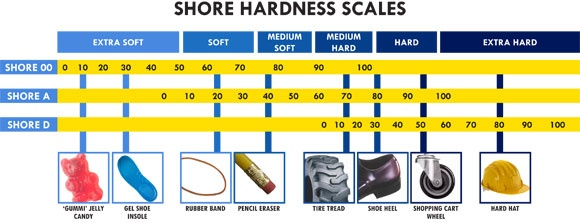
\includegraphics[width=\linewidth]{gfx/durometer}
	\caption[Shore hardness scales and everyday examples]{Shore types A, D, and OO in comparison with everyday examples of various hardnesses.\cite{smoothon-web}}\label{fig:shore}
	%http://www.smooth-on.com/images/durometer_with_logo_small_580.jpg
	%TODO use pdf instead of shitty jpg
\end{figure}

The silicone rubbers used for casting bracelet prototypes are both located on the Shore A scale. The softer Mold Star 15 Slow has a Shore A hardness of 15 that could be roughly compared to that of a rubber band according to figure \ref{fig:shore}, while the slightly harder Sorta-Clear 37 has a Shore A rating of 37, similar to that of a pencil eraser.%TODO cite datasheet

Both silicone products are two compound mixes that have to be added up and stirred before casting. While the Mold Star silicone has a rather low viscosity, casting the Sorta-Clear requires careful mold design, since it does not distribute well and is rather viscous. A vibrating table can help in filling the mold completely, but nonetheless were casts with the Sorta-Clear silicone much less fruitful, especially for the detailed molds of the one-piece designs (cf. section \ref{sec:silicone-prototypes}).

\section{Design Process and Prototype Manufacturing}
%Idea: Section as concepts like in the presentation: rigid prints, segmented prints, casts

The design process for the interactive bracelet presented in this thesis went through different stages. At first, a 3D-printed casing was favored, but later on a cast silicone bracelet turned out to be very comfortable for the user. The different prototypes are explained in detail in the following sections.

\subsection{Constant Thickness}

This very simple first approach is basically a rectangular profile rotated around a curve. It has the same magnitude at any point, which makes it quite uncomfortable to wear, especially under a layer of clothing.

\subsection{Tapered Shape}

With a tapered shape and non-uniform thickness, the bracelet looks more appealing. The reduced wall strength (0.7mm) made it very fragile in fabrication, two (out of two) prints broke during post-processing. Wearing the cuff while working on a PC feels only slightly uncomfortable, but twisting the hand is encumbered by the tight-fitting bracelet. Future prototypes should allow more space between the arm and the bracelet to ensure better comfort.

\subsection{Tapered Shape with Lid}

A modified design of Prototype 2 features a removable lid. The structure of the lid turned out to be too fine, especially the flexible part was too thin to work as intended. The size of the bracelet was increased a little to render it more comfortable to wear. Still, the rigid shape leads to clumsiness.

\subsection{Amico Bracelet Print-out}

A print of the tri-part design by Daniel Muschke on GrabCAD turned out to be a little too small, but the style felt more comfortable than the previous prototypes.

\subsection{Modified Tri-Part Design}

A re-work of Prototype 3 involves hinge research. The first draft turned out way too small, the second iteration was too big. Further research into this shape was paused because a long, bracelet-like display was considered instead of a small one.

\subsection{Silicone Bracelet}

After some consideration on a flexible, bracelet-shaped e-ink display, a prototype of silicone was considered. Mold design turned out a little tricky but finally succeeded. I printed a two-piece mold which only needed a little post-processing to fit properly together. The mold was coated with black spray paint to make the inside a little smoother, but this didn't work as intended so the paining step can be omitted in future mold making processes. The filling holes for the silicone were too small, and the silicone was more viscous than expected.

The first cast with a closed mold and filling through the holes was unsuccessful; it produced two small end pieces and nothing in between. For following casts, one part of the mold was filled with silicone and closed afterwards; this turned out significantly better. The orientation the mold is placed during dry period is also relevenat, as air bubbles will float towards the ``top'' of the mold, leading to instabilities. Getting the silicone part out of the mold was no problem.

The bracelet design involved a magnet clasp, but it was infeasible to strongly attach magnets to silicone with anything but silicone itself and they will likely jump out of place and snap together if placed closely in the design.

Two casts were made, one with each of the available silicone mixtures. The softer one was slightly too soft and had a disappealing color. As of yet, no tests have been conducted regarding the tightness of the display inside the bracelet.

\subsection{One-Piece Silicone Bracelet}
The next step was to cast a ring-like bracelet in one piece, so the issue with the clasp was no concern. The mold for this prototype consists of three pieces, two rings and a bottom plate. Unfortunately, the molds could not be recovered after the cast and had to be destroyed. In order to prevent unnecessary waste of material, the wall strength was reduced to 2.5 mm which turned out to be strong enough to survive the cast. However, one-time molds allow for tunnels in the display area.

This mold was much harder to fill with silicone than the previous one. Especially the Sortaclear silicone was too viscous to fill the complete mold, resulting in broken casts. The green Mold Star silicone turned out to work quite well.

\section{Touch slider}
The major input interface of the bracelet is a touch surface which consists of cut copper foil placed underneath the electrophorus display.
%TODO explain capacitive touch
%TODO explain geometry
%TODO explain interference sources
 